\documentclass[journal]{IEEEtran}
\usepackage[utf8]{inputenc}

\usepackage{graphicx}
%\usepackage[caption=false,font=footnotesize]{subfig}

\usepackage{url}
% Making the references and links clickable
\usepackage{hyperref}
\hypersetup{
	%colorlinks=false,
	pdfborder={0 0 0}
}

\usepackage{xcolor}
\newcommand{\toDo}[1]{\textcolor{red}{#1}}

\usepackage{fancyhdr}
\pagestyle{fancy}
\lhead{University of Brasília}
\rhead{\thepage}
\cfoot{Comparing the Performance of Finite-State Machines with Different Numbers of States on TORCS}
\renewcommand{\headrulewidth}{0.4pt}
\renewcommand{\footrulewidth}{0.4pt}

\begin{document}
	\title{Comparing the Performance of\\Finite-State Machines with\\Different Numbers of States on TORCS}
	
	\author{\IEEEauthorblockN{Bruno H. F. Macedo\IEEEauthorrefmark{1},
			Gabriel F. P. Araujo\IEEEauthorrefmark{1},
			Gabriel S. Silva\IEEEauthorrefmark{1},\\
			Matheus C. Crestani\IEEEauthorrefmark{1},
			Yuri B. Galli\IEEEauthorrefmark{1} and
			Guilherme N. Ramos\IEEEauthorrefmark{1}\IEEEauthorrefmark{2}\\[0.2cm]}
		\IEEEauthorblockA{\IEEEauthorrefmark{1}University of Brasília}
		\IEEEauthorblockA{\IEEEauthorrefmark{2}gnramos@unb.br}}
	
	\maketitle
	
	\begin{abstract}
		
		This work presents two different approaches developed to control a self-driving car in the racing environment
		simulated by TORCS. The problematic revolves around the representation of the complex behaviour that
		describes a pilot during a race, whose proposed solution is a finite-state machine. \toDo{Reduzir}The first method models
		the problem with states that separate the full driving behaviour into smaller fragments, thus simplifying the
		analysis and permitting parallel optimization; whilst the second method reduces the number of states with the
		objective of improving the performance, which is done by attenuating the impact that the function that
		manages the transition between states has on the controller as a whole. Furthermore, in order for the final
		controller to attain competitive status, i.e. parameter fine tuning, the incorporation of a genetic algorithm
		was performed. Evolving the driver using this method initially required the definition of a set of parameters
		to be the target of optimization, which would constitute the search space of the 
		
		
		Evolving the driver using Genetic Algorithm passed by defining the set of parameters 
		which would be the target to be optimazed, it initializion, random attributes insertion, evaluetion fuction 
		which provide a score, value that determine how good the parameters is.\toDo{Falar como foi, sucintamente,
		o processo de evolução com o Algoritmo Genético(é o suficiente?)}
		Validation\toDo{evaluetion?} occurred through exhaustively testing the configurations of the two approaches, comparing them
		along with artificial intelligences provided by the platform and also State of the Art implementations.
				
	\end{abstract}
	
	\begin{IEEEkeywords}
		
		finite state machines, computer games, TORCS, artificial intelligence, genetic algorithms, self-driving car
		\toDo{Finish keywords}
		
	\end{IEEEkeywords}
	
	\section{Topics}%
	
		Talk about:
		
		\begin{itemize}
			\item How the problem appeared;
			\item The approach chosen to solve it;
			\item How we evolved it by applying a genetic algorithm;
			\item How we improved the process of evolving through virus infection.
		\end{itemize}
		
		Include:
		\begin{itemize}
			\item State-of-art exposure;
			\item Model definition (theoretical outline);
			\item Test results;
			\item Results analysis;
			\item Prospects;
			\item Future works.
		\end{itemize}
		\newpage
	
	\section{\textbf{Introduction}} \label{sec:Intro}
	
	Automation of day to day tasks is an endeavour that has moved a large amount of scientific resources in the recent history~\cite{INDUS}~\cite{APPLI}. One specific example is target of research around the globe by a lot of universities, companies	and industries, which is the automation of vehicles, more specifically, automobiles. The objective of such attempts is the development of artificial intelligences capable of driving a car safely~\cite{SAFE}, with traffic law enforcement, real-time decision making, efficiency and, in addition, resource economy - as with gas, pollution emission~\cite{AUTOM} or even time. The practical applications of such controllers in autonomous vehicles are numerous, for example, the researches pursued by DARPA~\footnote{http://www.darpa.mil/our-research}.

	The Simulated Car Racing Championship (SCRC), using the platform TORCS (The Open Racing Car Simulator), has	brought an excellent environment for benchmarking AI approaches for the problem of autonomous car controllers~\cite{2009}. Even with the advent of computer simulations, finding the optimum behaviour of a car controller is a complex matter, so, many approaches have been suggested, such as heuristic algorithms~\cite{MrRacer} and modular and fuzzy architectures~\cite{AUTOPIA}. The strategy adopted in this work was to divide the problem into smaller portions, i.e., less complicated subproblems, in order to implement a finite-state machine that admittedly covers all necessary behaviours.
	
	One way to enhance the performance of the controllers created is by evaluating each and every possible set of parameters or configurations it could assume, but that choice is not always possible due to time and space complexities. Considering this, after an initial structure of the controller was designed, a method of computer-aided fine tuning was assimilated to it, which was a genetic algorithm.
	
	The rest of this Introduction is structured as follows: Section~\ref{sec:Environment} introduces TORCS, the working environment used in the problematic presented, along with the competition, SCR Championship, that currently represents the metric to evaluate the performance of controllers proposed for this environment; the section also presents what is already being done at this context in related works. Section~\ref{sec:FSM} then explains the proposal of the two developed controllers, clarifying their behaviour and structure, and briefly describing how they were augmented by the computer-aided method of a genetic algorithm. Section~\ref{sec:Experiments} describes how the validation process occurred through the methodology, the experiments and the results achieved, including their correspondent analysis. Section~\ref{sec:Conclusions} provides conclusions about the results acquired, which establish the comparison between the finite state machines with few and with moderate number of states, pointing out prospects about what might be done in future works to improve those results.

	\section{\textbf{The Simulation Environment}} \label{sec:Environment}

	\toDo{1. Why simulation}

	Simulations has used in multiples researches, such as in aviation industries~\cite{aviation}, medical education~\cite{medical}, robotic disaster response~\cite{VRC}. The aviation industry uses simulator to ... Medical colleges uses simulators to teach and evaluate the students, how to ... The Defense Advanced Research Projects Agency (DARPA) chose a simulation as process to evaluate which teams would continue in the challenge. Therefore a couple of reasons why we used simulations in this work:
	\begin{itemize}
		\item control and operational management;
		\item planning actions;
		\item understanding the problem and how to react;
		\item training and learning.
	\end{itemize}

	\toDo{2. Why TORCS as simulator}

	The Open Racing Car Simulator (TORCS) is a modern, modular, multi-player, multi-agent car simulator. A platform that is a widely used for benchmarking AI due its high degree of modularity and portability, concerning multi-platform environments - such as different operational systems - and support to the programming languages C and C++. Artificial intelligent agents can be developed into TORCS, as modules, there are many possibles levels of abstraction which can be evolved solutions. For example, at the car level, some intelligent control system for each car components. At the driver level, mid-level control systems to complex driving agents could be implemented using information - simulation state (partial) - given by a low-level API provided by TORCS.~\cite{TORCS}

	\toDo{3. How the simulation engine works}

	The TORCS engine uses a discrete-time simulation, the discretisation is set to 0.002s of simulation time. The engine solve differencial equations with Euler method and all basic elements of the vehicular dynamics is handled. Wich are

	\begin{itemize}
		\item basic properties of the vehicular system;
		\item mechanical details;
		\item dynamic and static friction;
		\item aerodynamic model.
	\end{itemize}

	Mass, rotational inertia of the car, engine, wheels and others components are included in the model of the vehicular system. The types of different suspension, links and differentials in the mechanical model. The profile for different ground types with each dynamic and static friction are included too. The aerodynamic includes slipstreaming and ground effects. Nevertheless the simulation engine can be replaced or easily modified owing the modularity of the TORCS.



	The Open Racing Car Simulator (TORCS) is a platform that is a widely used for benchmarking AI, renowned for its highly credible physics modeling engine and yet user-friendly interface for car racing simulation~\cite{TORCS}. One of the	many other qualities of this open-source simulator is its portability, concerning multi-platform environments - such as different operational systems and architectures - and support to the programming languages C and C++.

\subsection{TORCS} \label{subsec:TORCS}
	
	TORCS is a computer simulation that serves both as an ordinary car racing game and as a research platform~\cite{2009}, making it possible for everyone to create a pilot through coding. The interface with this platform occurs by means of a sensor-based interaction system in which the developer is able to interpret received parameters of the car - such as speed in X, Y and even Z axes - and control the car through programming its actuators, some of which are acceleration and steering.
	
	Another credibility factor for this platform is its non-punctual cars, which interact with each other in the races by a life-like collision system. Nevertheless, TORCS is still a simulator, and its limitations, along with the defined racing environment and the modeled car, are more than likely to affect any results obtained. This is an inherited characteristic of any real-life problem simulation, what in academia is denominated \emph{reality gap}~\cite{RG}, and it stems from the simplifications made concerning the car models, the technical features of the tracks, and so forth.

\subsection{The SCR Championship} \label{subsec:SCRC}

	The Simulated Car Racing Championship (SCRC) is an example of a well-known competition which utilizes TORCS as interface~\cite{SCR}. Being an event joining three competitions held at major scientific conferences, such as \emph{IEEE Congress on Evolutionary Computation}~\footnote{http://www.cec2015.org/}, \emph{Genetic and Evolutionary Computation Conference}~\footnote{http://www.sigevo.org/gecco-2015/} and \emph{IEEE Conference on Computational Intelligence and Games}~\footnote{http://www.ieee-cig.org/}, it is an accepted metric of evaluation in the fields of Evolutionary Computation and Computational Intelligence regarding Games.
	
	In the SCRC, some of the information about the racing execution remains hidden from the controllers, such as the geometrical format of the track and its category. The communication between this championship and TORCS is made through a client-server interface, with each player receiving information from the server regarding the sensors of the car, and in return providing actuator values that determine how the controller is supposed to drive the car. Figure~\ref{Fig:1} illustrates the data available at the TORCS and client - controller - layer of abstraction.

   	\begin{figure}[h]
		\centering
		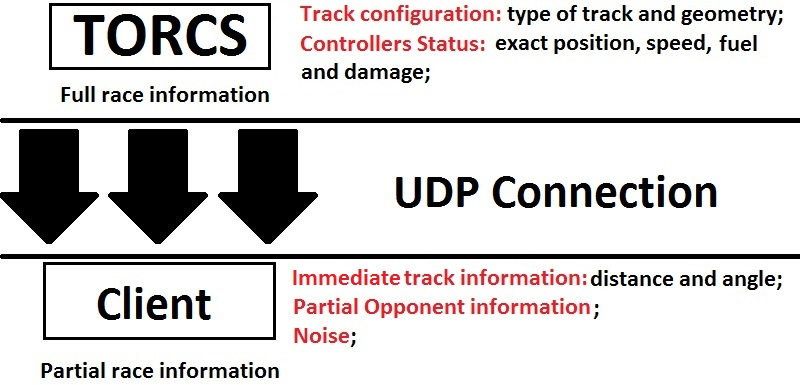
\includegraphics[width=250pt]{Figure1}
		\caption{\label{Fig:1}Available data inside TORCS and at the client.}
	\end{figure}
	
	The complete sensorial input information can be found at the Simulated Car Racing Championship Competition Software Manual~\cite{SCRC}. Noise can be introduced in the sensors, option that is present during the actual competition.

	Race tracks are categorized into \emph{Road}, \emph{Dirt} and \emph{Oval} inside TORCS. The races from the SCRC take place in track types decided by the organization of the championship, information which is not provided to the participants and that may incorporate maps that are unknown to them. The competition adopts a structure that gathers a \textit{Warm-up} stage, a \textit{Qualifier} stage and a \textit{Final} race, which are described in detail in a website of the competition~\cite{SCRC}.
	
	The reason why TORCS presents itself as a satisfactory AI benchmark, in combination with SCRC, is because even	though there are multiple possibilities on how the sensorial input received from the server can be translated into the behavior of the actuators, they can all be compared in a race, which has a robust and steady scoring and evaluational system. In other words, there are many different approaches concerning how to teach the racer encoded by the developers to drive in a racing competition only with the information given by the sensors, and the metric to that issue is the performance on the race itself.

\subsection{Related Works and State of the Art} \label{subsec:Related}
	
	It is very common among some of the SCRC awarded controllers the incorporation of machine learning in their driving methods, along with other evolving techniques using artificial intelligence. As the nature of the problematic presented comprises evolution by experience, learning procedures tend to enhance performance and competitiveness. Essentially, there are two ways of evolving controllers: Online Learning and Offline Learning, the first meaning that improvements are achieved during the actual race execution time and the latter that it is done after it, on the account of the developers themselves and with their own resources by analyzing the data gathered.
	
	The current champion of the SCR Championship is the controller \emph{Mr. Racer}~\cite{MrRacer}, and it has proven to be the State of the Art by winning the last three competitions that happened from 2011 to 2013. The authors of this implementation employ several heuristics and black-box optimization methods in order to reproduce the mechanisms to which human racing drivers resort, doing so by means of a modular structure. \emph{Mr. Racer} uses a Covariance Matrix Adaptation Evolution Strategy (CMA-ES), to evolve parameters offline.
	
	According to the founders of the competition~\cite{SCRC} and the authors of \emph{Mr. Racer} themselves, \emph{AUTOPIA}~\cite{AUTOPIA} is another competitive controller, with the potential to even be the best one available. \emph{AUTOPIA} implements a modular Fuzzy Architecture, whose division contains gear, steering and speed control; and it is optimized by means of a genetic algorithm for Offline Learning, and by means of landmarking the lane exit points for further speed reduction for Online Learning.
	
	These and other controller exemplifications~\cite{SCRC} served as criteria for the analysis and development of the approach presented in this paper. Aspects incorporated and adapted from them feature modularity, offline learning through genetic algorithms, online earning through landmarking and choosing sets of parameters for different categories of tracks, etc. Aspiring to design a controller capable of incorporating these features, the design of a model was proposed and is presented in the succeeding section.
	

	\section{\textbf{Related Works}} \label{sec:relworks}
	
		The reason why TORCS presents itself as a satisfactory AI benchmark is because there is an infinity of
		possibilities on how the sensorial input received from the server will be translated into the behaviour of the
		actuators, and they can all be compared in a race, which has a robust and steady scoring system. In other
		words, there are many different approaches concerning how to teach the racer encoded by the developers to
		drive in a racing competition only with the information given by the sensors, and the metric to that issue
		is the performance on the race itself.
		
		By controller, let it be understood that the subject is the programming code that in fact controls the
		car/driver/racer within racing environment. Some examples of awarded controllers and their driving methods
		will be presented in this section. They are what can be called the State of the Art among TORCS, and it is
		very common among them the incorporation of machine learning methods, along with other evolving techniques
		using artificial intelligence. Instinctively, as the nature of the problem comprises evolution by experience,
		learning procedures tend to enhance performance and competitiveness. Essentially, there are two ways of
		evolving controllers: Online Learning and Offline Learning, the first meaning that improvements are achieved
		during the actual race execution time and the latter that it is done before the competition, on the account of
		the developers themselves and with their own resources.
		
\subsection{State of the Art}
		
		The current champion of the SCR Championship is the controller \emph{Mr. Racer}~\cite{MrRacer}, and it has
		proven to be the State of the Art by winning at least the last three competitions that happened. The authors
		of this implementation learn parameters offline through Covariance Matrix Adaptation Evolution Strategy
		(CMA-ES), use regression and low-pass filtering to reduce noise impact, distinguish normal asphalted roads
		from dirt-based ones for behavioral separation and implement an authentic opponent-handling method. Their
		Online Learning consists on the track model selection to categorize into dirt or asphalt, choice of databased
		sets of parameters that best fit the track and the tuning of a target speed for all its corners.
		
		Another renowned controller is \emph{AUTOPIA}~\cite{AUTOPIA}. According to the founders of the
		competition~\cite{SoA} and the authors of \emph{Mr. Racer} themselves, it is a competitive match, with the
		potential to even be the best one available, but since no entries were received from them in a while, their
		means of winning a competition were somewhat restrained. Nevertheless, assessing its performance is
		worthwhile, and its description is the implementation of a modular Fuzzy Architecture, whose division contains
		gear, steering and speed control. Their controller is optimized by means of a genetic algorithm for Online
		Learning, and by means of landmarking the lane exit points for further speed reduction for Offline Learning.\toDo{verificar os termos offline e online}
		
		\toDo{Nós vamos	comparar o nosso piloto com o AUTOPIA? Se sim, devemos dizer isso aqui.}
		
		These and other controller exemplifications served as parameters for the analysis and development of the
		approach presented in this paper. Aspects incorporated and adapted feature modularity, offline learning
		through genetic algorithms, online learning through landmarking and choosing sets of parameters for different
		categories of tracks, etc. \toDo{Adicionar o quê mais fizemos no projeto como pincelada inicial para fazer o
		gancho com a seção Controller Structure.}
	\section{\textbf{FSMDriver - Controller Structure}} \label{sec:fsm}

	\subsection{First Approach - A Finite-State Machine With Five States}
	
	According to Mat Buckland in \emph{Programming Game AI By Example}~\cite{AI}:
	
	\begin{quotation}
		
		\emph{
		``A finite state machine is a device, or a model of a device, which has a finite number of states it can be in
		at any given time and can operate on input to either make transitions from one state to another or to cause
		an output or action to take place. A finite state machine can only be in one state at any moment in time.''}
		
	\end{quotation}
	
	Some of the main aspects desired to idealize a controller for TORCS were sufficed by the concept of	finite state
	machines~\cite{FSM}, the most important one being the goal of reaching an autonomous driving behaviour in a car
	race. This architecture was chosen in order to transform the problem of complex driving into smaller problems of
	situations found within the racing environment. Initially, the design of the finite-state machine proposed
	comprised the following states:
	
	\begin{itemize}

	\item \emph{Straight Line};
	\item \emph{Approaching Curve};
	\item \emph{Curve};
	\item \emph{Out of Track};
	\item \emph{Stuck}.

	\end{itemize}
	
	Essentially, for this method, normal behaviour covered \emph{Straight Line}, \emph{Approaching Curve} and
	\emph{Curve}, as the controller was located inside the track boundaries and no recovery actions needed to be
	considered, whereas exception behaviour consisted of \emph{Out of Track} and \emph{Stuck}, situations in which
	such conduct was expected. Here, a consideration needs to be taken into account: the real first model of the
	finite-state machine did not have an \emph{Approaching Curve} state, but, as the interpretations of the demeanour
	concerning the \emph{Straight Line} and the \emph{Curve} were so different from one another, a preparation had to
	be established so as to smoothen the transitions between them.
	
	If the controller was currently in \emph{Straight Line}, it would be expected of him to simply go as fast as he
	could, with no steering changes whatsoever; when in \emph{Approaching Curve} state, he would reposition himself
	in relation to the track and recalibrate his speed in order to make better curves; or, when in situations of
	\emph{Curve}, the pilot would reduce speed proportionally to the curvature of the curve, and then redirect
	himself towards the sensor pointing the biggest distance value read - which represents the direction of the curve.
	For the exception states, even though the expected deportment is well known, e.g. a stuck controller should
	maneuver the car out of the current situation and proceed to normal race conduct, the implementations vary among
	developers. The strategy chosen for the exception states was used on both proposals as a matter of regularity of
	comparison, and is explained on the next subsection.
	
	One big problem about this way of treating the matter is that the function responsible for choosing which state
	is more appropriate for each situation would more than often be overcharged, and, in some cases, rather different
	sets of parameters received by it would result in the same classification among the states. Thus, in order to
	minimize the dependency of the driving performance in relation to the function in charge of the transition
	between states, a project decision was made to reduce the number of states.
		
	\subsection{Proposition - A Finite-State Machine With Three States}
	
	The very nature of the initial architecture gave rise to the new approach. As mentioned within this very section,
	three of the states were innately part of a common bigger state, thereby \emph{Straight Line},
	\emph{Approaching Curve} and \emph{Curve} summed into \emph{Inside the Track}, resulting in the new controller
	with only three states, which were:
	
	\begin{itemize}
		
		\item \emph{Inside the Track};
		\item \emph{Out of Track};
		\item \emph{Stuck}.
		
	\end{itemize}
	
	\emph{Inside the Track}, therefore, is how the car, desirably, will spend most part of the time. The controller
	assumes a position of increasing the speed while steering towards the sensor with the biggest read value. This
	state also brakes, if necessary, when approaching turns.
	
	\emph{Out of Track} is when, for any unknown reason, the car is found outside of the track limits. In this case,
	the proper behaviour is to try to return to the lane. In road tracks, the outside track normally has a different
	terrain, sometimes dirt-based, meaning that skidding frequently occurs, and in a effort to avoid this, a control
	system to brake when the car begins skidding above a threshold was implemented.
	
	\emph{Stuck} represents any given situation that the car is unable to progress in the race. This is a delicate
	state, because it presents itself as difficult to identify and also due to its impact to the performance of the
	controller. In order to detect \emph{Stuck} circumstances, the speed of the car is monitored throughout the race,
	during every game tick, if it lingers with a low speed for a determined period, then it is considered stranded,
	or stuck. When detected, this state activates the reverse gear of the car and turns it until its front is
	directed towards the correct axis of the track. The reason why \emph{Stuck} is a sensitive state is because, when
	detected early, might indicate false positive, and when detected late, could lessen the efficiency of the
	controller. Thusly, detecting \textit{Stuck} situations is crucial, and so is handling the car out of them.
	
	In conclusion, each state in this manner of dealing with the process becomes, ideally, an independent problem,
	whose solution can be attacked separately. This way, they can all have individual sets of parameters susceptible
	to improvement, which will be discussed in the next section.
	\section{Genetic Algorithm}
	Due to the quantity of parameters to be tuned and the defined granularity, the space search is enormous and it's necessary some space search algorithm. In this study was chosen a evolutionary algorithm.
	
	
	A genetic algorithms are adaptive heuristic search algorithm based on the evolutionary ideas of natural selection. Genetics algorithms applications are present at many areas such as control engineering at non-linear system identification, biomedics to develop legs mechanism to proteses and even economy to forecast the behavior of agents.  
	
	Each individual is a string that contain the information necessary to evaluation. Usually, the values that composes the strings are parameters to be tuned. The search space of the optimization of parameters is defined by the representation of the chromosome.
		
	
	A randomly initial population is created, than, accordingly with the fitness function, is associated a score for each individual that represents how good the individual is.	
	
	
	Based on the premise that the better ones is more likely to reproduce a better offspring than others, the parents are chosen by the score of each individual. Thus your genetic material can be spread.
	
	
	To increase a genetic diversity each chromosome has a tiny chance to be mutate, this avoid a fast convergence of the algorithm, trying not to be stuck in a maximum local.
	
	
	For the model with 5 states, it was necessary adjust 22 parameters, each state has a different quantity, including the \emph{transition} function, as follows:

	\emph{Approach Curve} has 4 parameters.

	\emph{Transition Function} has 3 parameters.

	\emph{Straight Line} has 4 parameters.

	\emph{Out of Track} has 7 parameters.

	\emph{Stuck} has 4 parameters.
	
	
	

	\section{Methodology and Experiments} \label{sec:exp}
	Once defined the model and what parameters has to be tuned. In order to find the best configuration of parameters of the controller designed it was use a genetic algorithm.
	
	To find a general controller with good results for any track, the controller is evaluate with relation it's performance in various track, including dirt tracks and road tracks. 
	
	Due to the differences between dirt track and road tracks, it was made a two isolated evolution of controller, the first only on road tracks and the other one only on dirt tracks.
	
	Each individual race alone in a list of tracks, and the sum of the distance raced in the firstly 10000 cycles of time in each track is the fitness of the individual.
	
	In the end of evolution there will be pass more than 600 generations, each generation with 30 individuals.
	
	% needs review, just throwing ideas
	In order to find the best set of parameters for a general track the two machines states were evolved in three different set of tracks, one with 4 dirty tracks, one with 4 road tracks and another with the 4 of each type. 
	For the sake of comparison all the six controllers were tested in a predefined set of tracks, different from those where they were evolved.
	% the set of tracks was defined by autopia
	% tracks image as in the autopia's article
	The evaluation method used in the evolution was based on the qualifying stage of the SCRC, where each driver races alone for 10000 game ticks and those with the greater distance covered are selected.
	%add tables with the evaluation results
	
	
	%
	\section{Analysis and Conclusion}

	
\label{sec:concl}


	\section{Future Works} 	
	\begin{itemize}
		 \item Since at the SCRC the controller is allowed to perform a warm-up before the race it is possible to acquire the track data, not only mapping critical section such as sharp curves and points where the car go out the track to improve the result of the controller at the race itself. Also a warp-up stage would supply the information about environment where the car is, including the type of track,road or dirt, which determine a set of parameters best fitted to which occasion. 
        
		\item One important task to be accomplish is the opponent treatment, routines to reduce collisions, avoid the controller to be surpassed and surpass the opponents is a fundamental issue. Ignoring the opponent would make the driver to face unexpected collisions ending stuck, considering the worst event.
	\end{itemize}
	

	

	
	%\nocite{*}
	\bibliographystyle{IEEEtran}
	\bibliography{Bibliography}
	\toDo{Adequar as referências ao padrão do IEEE: \url{http://www.ieee.org/documents/ieeecitationref.pdf}. Quando
	há 3 ou mais autores colocar et al.}
	
	
	
\end{document}
